\documentclass{article}

\usepackage[T1]{fontenc}
\usepackage{graphicx}
\usepackage{fancyhdr}
\pagestyle{fancy}
\fancyhf{}
\lhead{Draft 0.1}
\rhead{Elliot Oram}
\rfoot{\thepage}


\title{Staging Area Design}
\author{elo9@aber.ac.uk}

\begin{document}

\maketitle
\tableofcontents

\newpage

\section{Staging Area: Top Down}
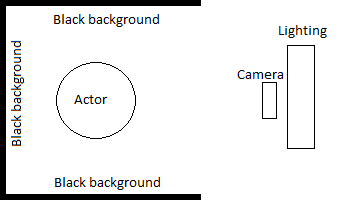
\includegraphics[width=\textwidth]{TopDown}
\section{Staging Area: Side View}
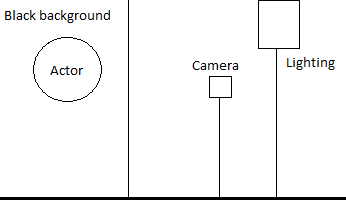
\includegraphics[width=\textwidth]{SideView}

\newpage


\section{Staging area components}
\begin{itemize}
	\item \textbf{Actor}\\
	\textbf{Location} - Centre of staging area \\
	\textbf{Description} - The Actor will be performing activities in the staging area. These will be filmed by the camera, processed and displayed as a hologram in the Viewing Area.
	
	\item \textbf{Black background}\\
	\textbf{Location} - Surrounds the actor and forms the edge of the Staging Area\\
	\textbf{Description} - The black background which will be free-standing hardboard (or similar) is used for the background of the video. The back panel behind the Actor will be the background and the side panels will help to reduce light pollution from the rest of the room.
	
	\item \textbf{Camera}\\
	\textbf{Location} - In front of the open side of the black background panels. The camera must be positioned far enough away from the actor to capture the full body.\\
	\textbf{Description} - The camera will capture the movements of the Actor and will be attached to the image processing machine as an external peripheral. 
	
	\item \textbf{Lighting}\\
	\textbf{Location} - The lighting rig will be positioned behind the camera and mounted to be above the Actor and camera \\
	\textbf{Description} - The lighting rig will consist of one bright light covered with a soft box to diffuse the light. The light will be pointed at the Actor and the unwanted contribution it makes to illuminating the background, will be removed by the image processing application.

\end{itemize}

\section{Further considerations}
The height of the black background needs to be enough that it removes contributions from the environment. At present, the design does not include a top. This should not be a problem as, whilst the sports hall (where science week is normally held) does have overhead lighting, the background subtraction in the image processing application will account for this.

\end{document}